\documentclass[titlepage,11pt]{article}
\usepackage{graphicx,setspace,fancyvrb}
\usepackage[left=2cm,top=2cm,right=2cm,bottom=1cm,nofoot]{geometry}

\begin{document}
\onehalfspacing



\begin{singlespacing}
\title{Determining Appropriate Phosphorus Discharge in a Stream}
\author{Cameron Bracken\\Humboldt State University\\ENGR 326}
\date{\today}
\maketitle
\newpage
\begin{abstract} The effluent of a wastewater treatment plant
contained phosphorus which was discharged at a fixed rate.  A
community was faced with a new water quality standard for the
phosphorus concentration in the stream at a downstream test site.  A
model was proposed relating the rate of decay of the phosphorus
concentration to the algal growth rate by a system of ordinary
differential equations. The Runge-Kutta-Fehlberg method combined
with a step size control algorithm was used to determine the
phosphorus concentration at the downstream test site. A sensitivity
analysis also showed which parameters had the greatest affect on the
model output.  The model determined that the rate of phosphorus
discharge needed to be greatly decreased in order to meet the water
quality standard at the test site.
\end{abstract}

\pagenumbering{roman}\pagestyle{myheadings}
\tableofcontents\addcontentsline{toc}{section}{List of Figures}
\listoffigures \addcontentsline{toc}{section}{List of Tables}
\listoftables
\newpage
\end{singlespacing}
\pagestyle{headings}\pagenumbering{arabic}

\section {Introduction}
A community is currently discharging 0.85 mg/l of phosphorus into a
local stream. For recreation and domestic purposes, a new standard
is imposed which calls for the phosphorus concentration to be less
than 0.05 mg/l at a monitoring point 43.2 km downstream (Finney
2006). The purpose of this report is to determine:
\begin{itemize}
\item{the current concentration of phosphorus at the monitoring point.}
\item{how much treatment (if any) is needed to
bring the phosphorus concentration below 0.05 mg/l at the monitoring
point.}
\end{itemize}

\section{Methodology}
Phosphorus concentration in the stream declines due to sedimentation
and algal uptake.  Algal growth is limited by the amount of
phosphorus available.  The algal growth rate (and phosphorus decline
rate) is described by
\begin{eqnarray}
\frac{dP}{dt}&=&K_{P_1}P-K_{P_2}\mu A\\
\frac{dA}{dt}&=&-K_{A_1}A-\mu A
\end{eqnarray}
where
\begin{singlespacing}
\begin{center}
\begin{tabular}{rcl}
$P$&=&phosphorus concentration (mg/l)\\
$A$&=&chlorophyll-A concentration (algae)(mg/l)\\
$t$ &=&time (days)\\
$K_{P_1}$ &=&first order removal rate of phosphorus (1/day)\\
$K_{P_2}$ &=& yield coefficient (mg phosphorus/mg chlorophyll-A\\
$K_{P_3}$ &=& half saturation concentration for phosphorus (mg/l)\\
$K_{A_1}$ &=& algal death rate (1/day)\\
$\mu$ &=& algal growth rate (1/day)\\
 &=&$\mu_{max}\left(\frac{P}{K_{P_3}+P}\right)$\\
$\mu_{max}$ &=& maximum algal growth rate
\end{tabular}
\end{center}
\end{singlespacing}

To determine the concentration of phosphorus 43.2m downstream, the
system of ordinary differential equations (ODEs), Equations 1 and 2,
must be solved for P.  The solution will yield P(t) and A(t), which
can be easily converted to P(d) and A(d) where d is the distance
downstream.

An analytical solution to the system of Equations 1 and 2 is not
easily obtained so a numerical method must be used to produce a
solution. A Runge-Kutta-Fehlberg (RKF) routine paired with a step
size control algorithm is is a sufficiently robust method to solve
the ODEs and mitigate error.  On every iteration, the RKF routine
computes a fourth and
fifth order Runge-Kutta method estimate.\\\\
$$y_{fourth_{i+1}}=y_{fourth_{i}}+\left(\frac{37}{378}k_1+\frac{250}{621}k_3+
\frac{125}{594}k_4+\frac{512}{1771}k_6\right)h$$
$$y_{fifth_{i+1}}=y_{fifth_{i}}+\left(\frac{2825}{27648}k_1+\frac{18575}{48384}k_3+
\frac{13525}{55296}k_4+\frac{277}{14336}k_5+\frac{1}{4}k_6\right)h$$
where h is the step size and $k_i$ is a value between $t_i$ and
$t_{i+1}$.  Once computed, the fourth and fifth order estimates are
compared to find the relative error
$$\varepsilon_{rel}=\left|\frac{y_{fifth}-y_{fourth}}{y_{fifth}}\right|$$
The relative error ($\varepsilon_{rel}$) is used by RKF to control
the step size on the following iteration (Figure 1). The step size
control algorithm puts an upper and lower limit
($\varepsilon_1,\varepsilon_2$) on the relative error to prevent
inaccurate results and slow progress, respectively. A minimum and
maximum step size are also imposed for error checking purposes.

\begin{figure}[h] \label{fig:stop}
\begin{center}
\begin{Verbatim}[frame=single]
if(emax>eps2 .and. abs(h-hmin)>10d-6)then
  h=h/2                         !large error,reduce step size and try again
  y=ysave
else
  t=t+h                         !advance time, accept solution
  if(emax>eps2)exitflag=1       ! big error but h=hmin
  if(emax<eps1 .and. h<hmax)then
  h=h*2d0                       !small error increase step size
  if(h>hmax)h=hmax
  end if
  hsave=h                       !save the step size we are on
  if(t>=tend)exit               !are we done?
  if((t+h)>tend)=tend-t         !will the next step be beyond the end
end if
\end{Verbatim}
\caption{Step size control}
\end{center}
\end{figure}
\section{Application}

The concentration of phosphorus 43.2 km downstream is dependent on
various parameters that are known in the problem (Table 1).
\begin{table}[h]\label{tbl:param}
\begin{center}
\caption{Parameters associated with determining phosphorus
concentration}
\begin{tabular}{|l|l|l|}
\hline
{\bf Parameter} & {\bf Variable} & {\bf Value} \\
\hline
Settling rate of P  &  $K_{P_1}$&     0.05/day \\
\hline
Yield &      $K_{P_2}$ &  1.0 (dimensionless) \\
\hline
Half Saturation of P  & $K_{P_3}$  & 0.025 mg/l\\
\hline
Algal death rate & $K_{A_1}$ &  0.003/day \\
\hline
Maximum algal growth rate & $\mu_{max}$ & 0.42/day\\
\hline
Minimum allowable error & $\varepsilon_1$ & $1\times10^{-6}$\\
\hline
Maximum allowable error & $\varepsilon_2$ &
$1\times10^{-2}$\\
\hline
\end{tabular}
\end{center}
\end{table}

To test the sensitivity of the system, some parameters can be varied
(Table 2).

\begin{table}[h]
\begin{center}
\caption{Variation of Parameters for analyzing model sensitivity}
% Table generated by cameron
\begin{tabular}{|c|r|r|r|r|}
\hline
{\bf Run \#}& {\bf Variable}     &{\bf Initial value}& {\bf New value}   & {\bf Variation} \\
\hline
          1 &    $K_{P_1}$       &     0.05/day     &       0.045        &  -10\% \\
          2 &                    &     0.05/day     &       0.055        &   10\% \\
 \hline
          3 &    $K_{P_2}$       &        1.0       &         0.9        &  -10\% \\
          4 &                    &        1.0       &         1.1        &   10\% \\
 \hline
          5 &    $K_{P_3}$       &    0.025 mg/l    &       0.0225       &  -10\% \\
          6 &                    &    0.025 mg/l    &       0.0275       &   10\% \\
\hline
          7 &    $K_{A_1}$       &     0.003/day    &      0.0027        &  -10\% \\
          8 &                    &     0.003/day    &      0.0033        &   10\% \\
 \hline
          9 &    $\mu_{max}$     &      0.42/day    &      0.378         &  -10\% \\
         10 &                    &      0.42/day    &      0.462         &   10\% \\
\hline
         11 &  $\varepsilon_1$   & $1\times10^{-6}$ &  $5\times10^{-7}$  &  -50\% \\
         12 &                    & $1\times10^{-6}$ & $1.5\times10^{-6}$ &   50\% \\
\hline
         13 &  $\varepsilon_2$   & $1\times10^{-2}$ &  $5\times10^{-3}$  &  -50\% \\
         14 &                    & $1\times10^{-2}$ & $1.5\times10^{-6}$ &   50\% \\
\hline
\end{tabular}
\end{center}
\end{table}


\section{Results}

As the effluent moves downstream the phosphorus concentration
decreases and the algae concentration increases (Figure 2).  With
$P_0=0.85$ mg/l, program \verb maxeff  gives the phosphorus
concentration 43.2 km downstream as0.419 mg/l.  With an initial
phosphorus concentration of 0.85 mg/l the concentration at 43.2 km
is far above the standard of 0.05 mg/l.

\begin{figure}[h] \label{fig:avp}
\begin{center}
\scalebox{.52}{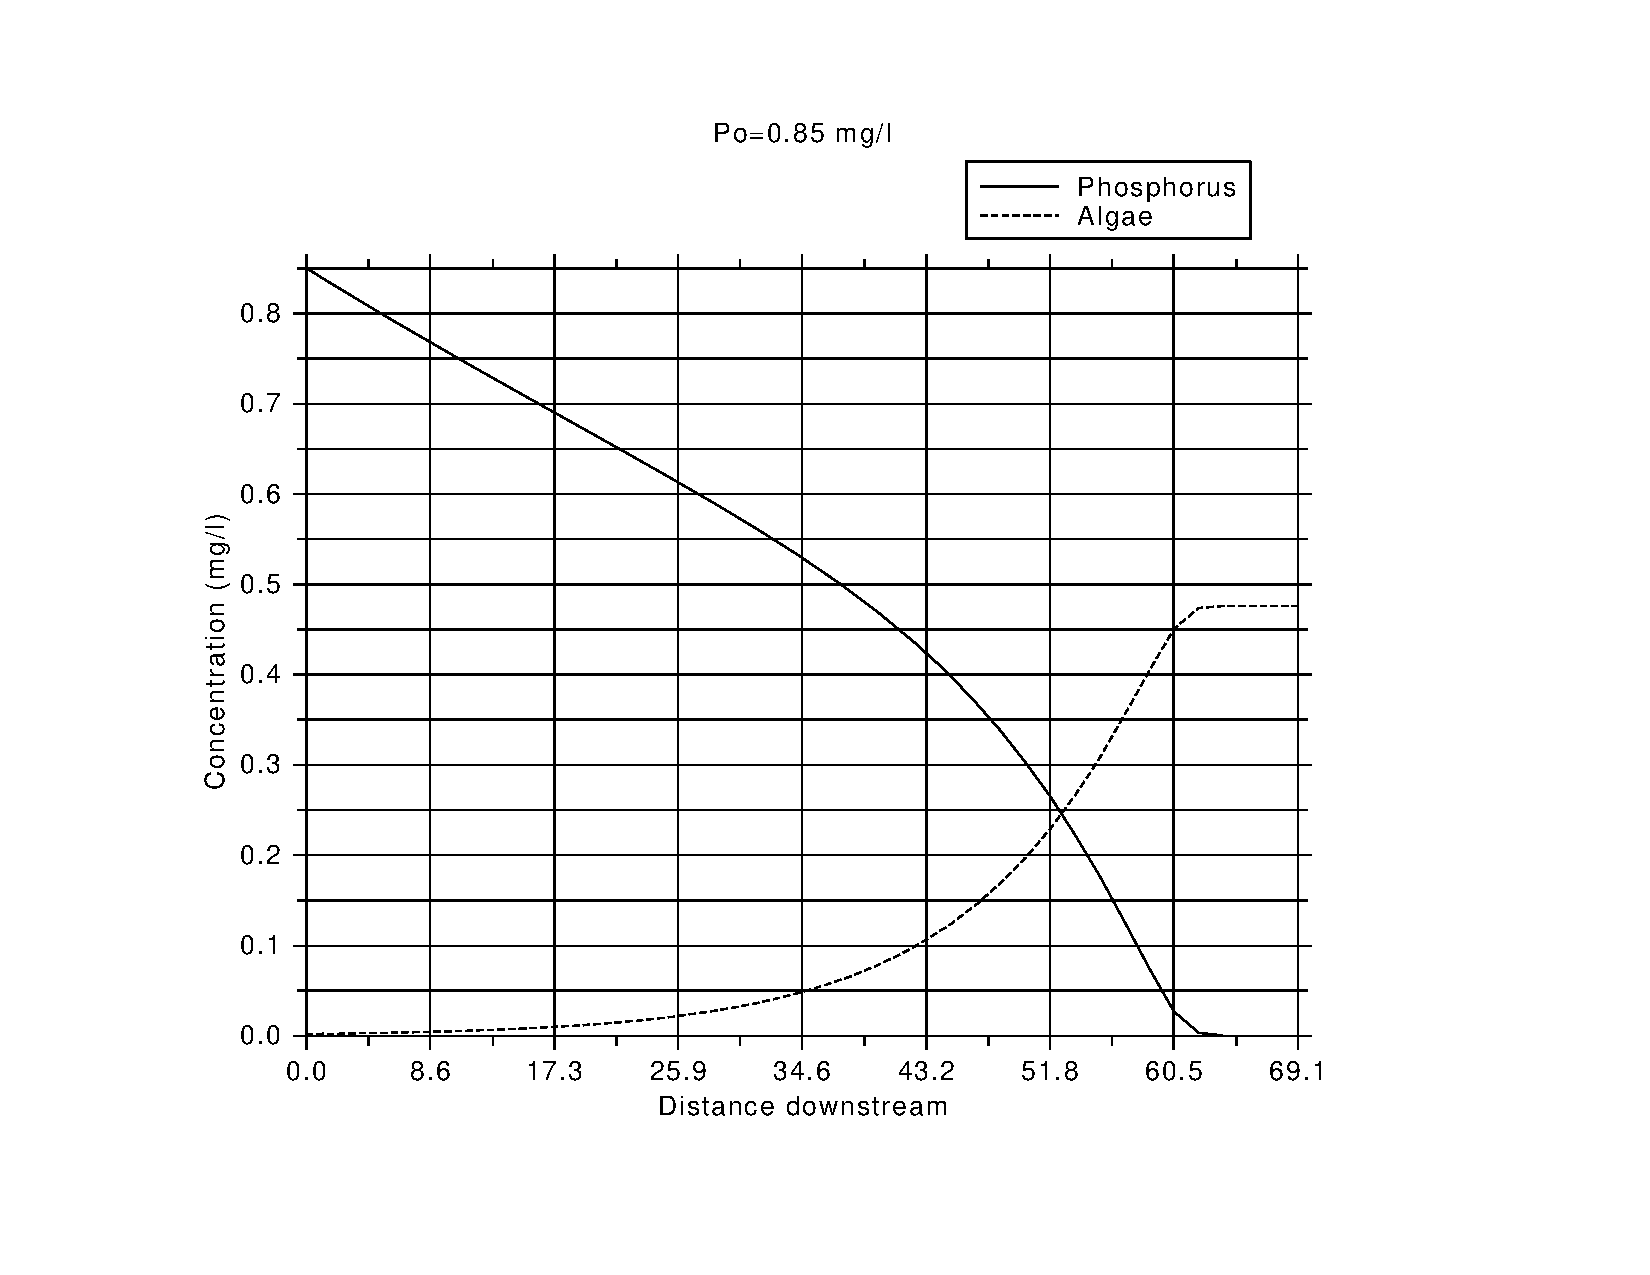
\includegraphics{dislin_1.pdf}} \caption{Solution
curves for untreated initial concentration.}
\end{center}
\end{figure}

\newpage The sensitivity analysis reveals how the downstream concentration
of phosphorus varies when individual parameters are varied.
Phosphorus concentration is most sensitive to changes in the maximum
algal growth rate ($\mu_{max}$) and least sensitive to changes in
algal death rate ($K_{A_1}$) (Table 3). Varying the maximum and
minimum allowable error also has a negligible effect on the
phosphorus concentration.

\begin{table}[h]
\begin{center}
\caption{Parameters associated with determining phosphorus
concentration}
% Table generated by Excel2LaTeX from sheet 'AcrD227'
\begin{tabular}{|r|r|l|l|l|l|l|}
\hline
{\bf Run \#} & {\bf Variable} & {\bf New value}  & {\bf \% varied} & {\bf P$_{43.2 km}$ (mg/l)} & {\bf Variation}\\
\hline
         1 &       $K_{P_1}$  &     0.045        &       -10\%          & 0.444                     &5.97\%\\
         2 &                  &     0.055        &        10\%          &0.396                      &5.49\%\\
\hline
         3 &     $K_{P_2}$    &       0.9        &       -10\%          &0.429                      &2.39\%\\
         4 &                  &        1.1       &        10\%          &0.410                      &2.15\%\\
\hline
         5 &       $K_{P_3}$  &    0.0225        &       -10\%          &0.418                      &0.24\%\\
         6 &                  &    0.0275        &        10\%          &0.421                      &0.48\%\\
\hline
         7 & $K_{A_1}$        &0.0027            &       -10\%          &0.419                      &0\%\\
         8 &                  &0.0033            &        10\%          &0.419                      &0\%\\
\hline
         9 &      $\mu_{max}$ &  0.378           &       -10\%          &0.452                      &7.88\%\\
        10 &                  & 0.462            &        10\%          &0.370                      &11.7\%\\
\hline
        11 &  $\varepsilon_1$ & $5\times10^{-7}$ &       -50\%          &0.419                      &0\% \\
        12 &                  &$1.5\times10^{-6}$&        50\%          &0.419                      &0\% \\
\hline
        13 & $\varepsilon_2$  &$5\times10^{-3}$  &  -50\%               &0.419                      &0\%\\
        14 &                  &$1.5\times10^{-2}$&  50\%                &0.419                      &0\%\\
\hline
\end{tabular}
\end{center}
\end{table}

To determine the level of treatment to impose at the discharge site,
different initial concentrations were tested (Table 4).  An initial
concentration of 0.16 mg/l will yield a downstream concentration
P=0.049, just below the standard (Figure 3).  To meet the standard,
the phosphorus concentration at the discharge point needs to be
decreased by 0.69 mg/l or 81.2\%.

\begin{figure}[h] \label{fig:curves}
\begin{center}
\scalebox{.65}{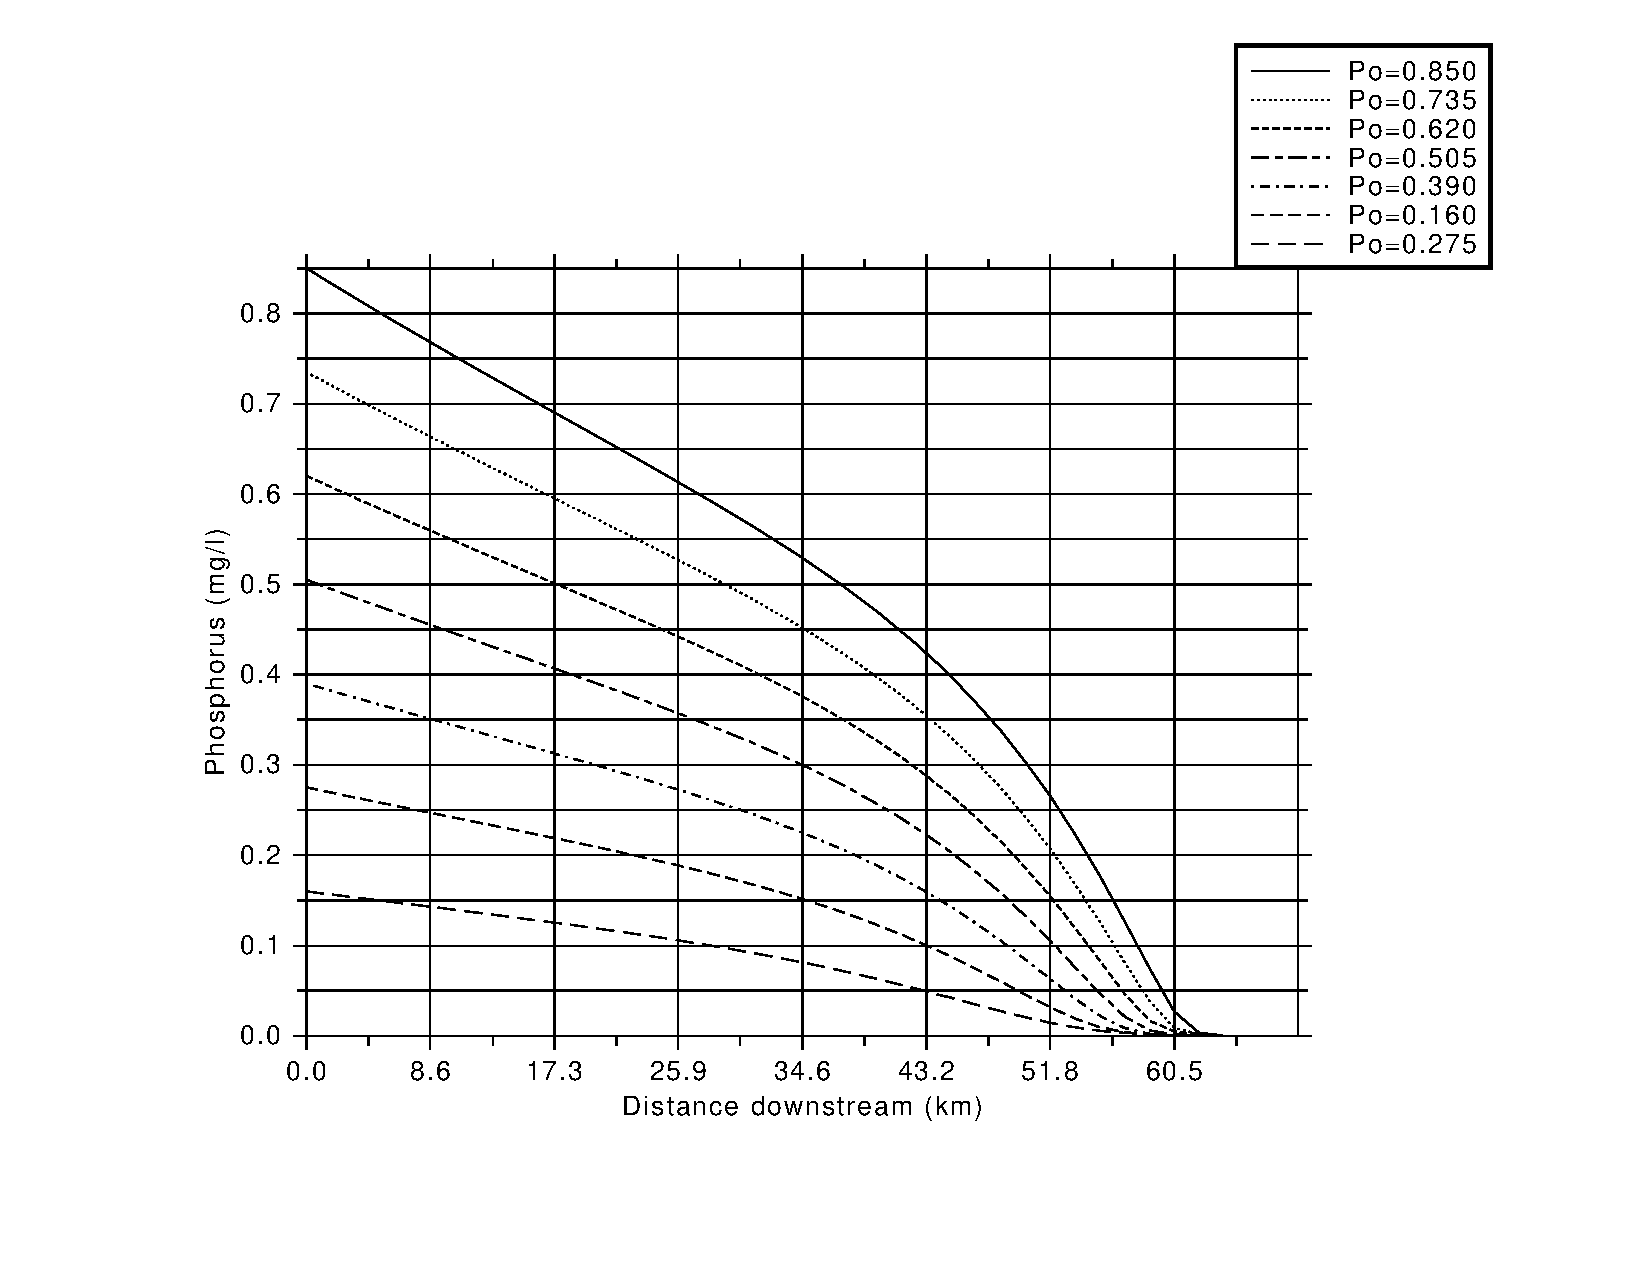
\includegraphics{dislin_4.pdf}} \caption{The bottom
curve shows an initial concentration that meets the standard 43.2km
downstream}
\end{center}
\end{figure}

\begin{table}[h]
\begin{center}
\caption{Initial conditions}
% Table generated by cameron
\begin{tabular}{|l|l|}
\hline
{\bf $P_0$}& {\bf $P_{43.2}$} \\
\hline
       0.85 &    0.419   \\
\hline
      0.735 &    0.352   \\
\hline
       0.62 &    0.286   \\
\hline
       0.50 &    0.221   \\
\hline
        0.39&    0.158   \\
\hline
       0.275&    0.100   \\
\hline
        0.16&    0.049   \\
\hline
\end{tabular}
\end{center}
\end{table}



%\break\clearpage\pagebreak
\newpage
\section{Conclusion}
The following can be concluded from the analysis:
\begin{itemize}
\item{The downstream concentration when $P_0$=0.85 will be P=0.419 mg/l.}
\item{Themodel is most sensitive to changes in $\mu_{max}$.}
\item{The model is least sensitive are to changes in
$K_{A_1}$,$\varepsilon_1$ and $\varepsilon_2$.}
\item{Under current conditions the standard of 0.05 mg/l will not be met.}
\item{An 81.2\% decrease in discharge is needed to meet the
standard.}
\end{itemize}

\section{References}
\noindent Finney,Brad. Lab 5 handout, Humboldt State University,
Fall 2006.

\appendix
\newcommand{\appsection}[1]{\let\oldthesection\thesection
  \renewcommand{\thesection}{Appendix \oldthesection}
  \section{#1}\let\thesection\oldthesection}
\appsection{\\~Source Code} \label{sec:source}
\begin{singlespacing}
\begin{small}
\begin{Verbatim}[frame=single]
module odec
  double precision::umax,kp1,kp2,kp3,ka1
end module odec


program maxeff
  use dislin
  use odec
  implicit none
  integer::neq,npts,exitflag,i,j
  double precision::deltat,h,hmin,hmax,tstart,tend,eps1,eps2,ans
  double precision,allocatable,dimension(:)::y,P,A,T
  character(len=8)::fn
  integer, parameter::maxn=100
  double precision::xa,xe,xor,xstep,ya,ye,yor,ystep
  character (len=10)::fmt="(a)"
  character (len=200)::legendstring

  interface
    subroutine rkf(tstart,tend,n,y,h,hmin,hmax,eps1,eps2,f,exitflag)
      double precision,dimension(:),intent(inout)::y
      double precision,intent(in)::hmin,hmax,eps1,eps2
      double precision,intent(inout)::tstart,tend,h
      integer,intent(inout)::exitflag
      integer,intent(in)::n
      interface
        subroutine f(t,y,Dy,exitflag)
          integer,intent(inout)::exitflag
          double precision,intent(in)::t
          double precision,dimension(:),intent(in)::y
          double precision,dimension(:),intent(out)::Dy
        end subroutine f
      end interface
    end subroutine rkf
    subroutine ode(t,y,Dy,exitflag)
      integer,intent(inout)::exitflag
      double precision,intent(in)::t
      double precision,dimension(:),intent(in)::y
      double precision,dimension(:),intent(out)::Dy
    end subroutine ode
  end interface

  !This program will solve a sysyem of  first order ODE's and
  !plot them using the dislin graphics package
  !also see lab5_dislin.f90
  !variable list
  !neq=       number of equations
  !npts=      number of output points
  !deltat=    distace between output points
  !tstart=    starting point for rkf routine
  !tend=      ending point for rkf routine
  !h=         step size for rkf routine
  !hmin=      minimum allowable step size
  !hmax=      maximum allowable step size
  !y=         solution vector at tend
  !P=         vector of phosphorus concentrations
  !A=         vector of chlorophyll-A concentrations
  !fn=        name of input file
  !exitflag=  error checking
  !eps1=      minimum allowable error
  !eps2=      maximum allowable error

  fn="vars.dat"
  open(11,file=fn)
  write(*,*)"How many points?"
  read(*,*)npts
  read(11,*)neq,h,hmin,hmax,eps1,eps2,umax,kp1,kp2,kp3,ka1
  allocate(y(neq),P(npts+2),A(npts+2),T(npts+2))
  deltat=200d0/dble(npts)                !fix intervals
  !deltat=60d0/dble(npts)                !for test ode
  y(1)=0.85d0
  y(2)=2d-3
  !y(1)=300                              !for test ode
  tend=0
  P(1)=y(1)
  A(1)=y(2)
  T(1)=tstart

  xa=0d0 ! xa is the lower limit of the x-axis.
  xe=69.11d0 ! xe is the upper limit of the x-axis.
  xor=0 ! xor is the first x-axis label.
  xstep=8.64 ! xstep is the step between x-axis labels.
  ya=0d0 ! ya is the lower limit of the y-axis.
  ye=.85d0 ! ye is the upper limit of the y-axis.
  yor=0 ! yor is the first y-axis label.
  ystep=.1d0 ! ystep is the step between y-axis labels.
  !Plot data using DISLIN
  call metafl("BMP") ! or "PS", "EPS", "PDF", "WMF" "BMP"
  call setpag("USAL") !"USAL" is US size A landscape, "USAP" is portrait
  call scrmod("REVERS") !sets black on white background
  call disini() !Initialize dislin
  call complx ! Sets the font
  call name("Distance downstream (km)","X") ! Set label for x-axis
  call name("Phosphorus (mg/l)","Y") ! Set label for y-axis
  call titlin("Phosphorus Concentrations",1) ! Set 1st line of plot title
  call psfont("Helvetica")
  call graf (xa, xe, xor, xstep, ya, ye, yor, ystep) ! sets up axis
  call title ! Actually draw the title in over the axis
  call grid(1,2)
  call legini(legendstring,7,8) ! Store 2 lines of legend text, max20 characters/line
  CALL LEGPOS(2205,0) !defines a global position for the legend where NX and NY are the
                  !plot coordinates of the upper left corner. After a call to LEGPOS,
                  !the second parameter in LEGEND will be ignored.
  call FRAME(5)
  call legtit("") ! set legend title (default="legend")
  call leglin(legendstring,"Po=0.850",1) ! Specify the legend text for curve 1
  call leglin(legendstring,"Po=0.735",2)
  call leglin(legendstring,"Po=0.620",3)
  call leglin(legendstring,"Po=0.505",4)
  call leglin(legendstring,"Po=0.390",5)
  call leglin(legendstring,"Po=0.275",6)
  call leglin(legendstring,"Po=0.160",7)

  do j=1,7
    tstart=0
    tend=0
    A(1)=y(2)
    P(1)=y(1)
    T(1)=tstart
    do i=1,npts+1
      tstart=tend                         !advance interval
      tend=tend+deltat
      call rkf(tstart,tend,neq,y,h,hmin,hmax,eps1,eps2,ode,exitflag)
      if(exitflag/=0)then
        write(*,*)"error"
        stop
      end if
      P(i+1)=y(1)
      A(i+1)=y(2)
      T(i+1)=4.32*(tend/10d0)
      if (T(i+1)>=43.2d0 .and. j==1)then
        ans=P(npts/2+1)
      end if
    end do
    call curve(T,P,npts+1) ! draw the x-y curve
    call lintyp(j) ! Change the line style (values are from 1 to 7)
    write(*,*)"Po=",.85-dble(j-1)*.115d0
    y(1)=.85-dble(j)*.115d0
    y(2)=2d-3
    write(*,*)"T=",T(npts/2+1),j
    write(*,*)"P=",P(npts/2+1),j
   end do
  call legend(legendstring,3) ! draw legend in 7 (upper right inside axis)
  !draw legend in location 1-8. 1-4=page corner, 5-8=axis corner,1 and 5=lowerleft
  call disfin ! finish off the plot
  write(*,*)"***",ans,"***"
end program maxeff


subroutine rkf(tstart,tend,n,y,h,hmin,hmax,eps1,eps2,f,exitflag)
  implicit none
  double precision,dimension(:),intent(inout)::y
  double precision,intent(in)::hmin,hmax,eps1,eps2
  double precision,intent(inout)::tstart,tend,h
  integer,intent(inout)::exitflag
  integer,intent(in)::n
  double precision,dimension(n)::K1,K2,K3,K4,K5,K6,Dy,y4,ysave
  double precision::t,hsave,emax
  double precision,parameter::c1=1d0/5d0,c2=3d0/10d0,c3=3d0/40d0,c4=9d0/40d0,&
            c5=3d0/5d0,c6=3d0/10d0,c7=-9d0/10d0,c8=6d0/5d0,c9=11d0/54d0,&
            c10=5d0/2d0,c11=-70d0/27d0,c12=35d0/27d0,c13=7d0/8d0,&
            c14=1631d0/55296d0,c15=175d0/512d0,c16=575d0/13824d0,c17=44275d0/110592d0,&
            c18=253d0/4096d0,c19=37d0/378d0,c20=250d0/621d0,c21=125d0/594d0,&
            c22=512d0/1771d0,c23=2825d0/27648d0,c24=18575d0/48384d0,&
            c25=13525d0/55296d0,c26=277d0/14336d0,c27=1d0/4d0

  interface
    subroutine f(t,y,Dy,exitflag)
      integer,intent(out)::exitflag
      double precision,intent(in)::t
      double precision,dimension(:),intent(in)::y
      double precision,dimension(:),intent(out)::Dy
    end subroutine f
    subroutine test(t,y,Dy,exitflag)
      integer,intent(inout)::exitflag
      double precision,intent(in)::t
      double precision,dimension(:),intent(in)::y
      double precision,dimension(:),intent(out)::Dy
    end subroutine test
  end interface

  !variable list
  !y=          solution vector
  !h=          step size
  !hmin=       minimum step size
  !hmax=       maximum step size
  !hsave=      save step size for end of interval
  !t=          current time
  !tstart=     start of time interval
  !tend=       end of time interval
  !n=          number of equations
  !Kn=         Runge Kutta constants
  !Dy=         Derivative estimate at current time
  !y4=         fourth order runge-kutta
  !emax=       error between fourth and fifth order estimates
  !exitflag=   error checking
  !eps1=       minimum allowable error
  !eps2=       maximum allowable error

  t=tstart
  exitflag=0
  if((t+h)>tend)then
    hsave=h
    h=tend-t
  end if
  do
    ysave=y
    call f(t,y,Dy,exitflag)
      if(exitflag/=0)return
      K1=h*Dy
    call f(t+c1*h,y+c1*K1*h,Dy,exitflag)
      if(exitflag/=0)return
      K2=h*Dy
    call f(t+c2*h,y+c3*K1*h+c4*K2*h,Dy,exitflag)
      if(exitflag/=0)return
      K3=h*Dy
    call f(t+c5*h,y+c6*K1*h+c7*K2*h+c8*K3*h,Dy,exitflag)
      if(exitflag/=0)return
      K4=h*Dy
    call f(t+h,y+c9*K1*h+c10*K2*h+c11*K3*h+c12*K4*h,Dy,exitflag)
      if(exitflag/=0)return
      K5=h*Dy
    call f(t+c13*h,y+c14*K1*h+c15*K2*h+c16*K3*h+c17*K4*h+c18*K5*h,Dy,exitflag)
      if(exitflag/=0)return
      K6=h*Dy
    y4=y+(c19*K1+c20*K3+c21*K4+c22*K6)*h
    y=y+(c23*K1+c24*K3+c25*K4+c26*K5+c27*K6)*h
    emax=maxval(abs((y-y4)/y))          !max relative truncation error
    if(emax>eps2 .and. abs(h-hmin)>10d-6)then
      h=h/2                             !large error,reduce step size and try again
      y=ysave
    else
      t=t+h                             !advance time, accept solution
      if(emax>eps2)exitflag=1           ! big error but h=hmin
      if(emax<eps1 .and. h<hmax)then
        h=h*2d0                         !small error increase step size
        if(h>hmax)h=hmax
      end if
      hsave=h                           !save the step size we are on
      if(t>=tend)exit                   !are we done?
      if((t+h)>tend)h=tend-t            !will the next step be beyond the end
    end if
  end do
  h=hsave
  return
end subroutine rkf

subroutine ode(t,y,Dy,exitflag)
  use odec
  implicit none
  integer,intent(inout)::exitflag
  double precision,intent(in)::t
  double precision,dimension(:),intent(in)::y
  double precision,dimension(:),intent(out)::Dy
  double precision::u

  u=umax*(y(1)/(kp3+y(1)))
  Dy(1)=-kp1*y(1)-kp2*u*y(2)
  Dy(2)=-ka1*y(2)+u*y(2)

end subroutine ode

Script started on Thu 12 Oct 2006 12:43:49 PM PDT
cwb12@ere-lab11:~/engr326/lab5> if90link -a -r8 lab5
 How many points?
50

 <<<<<<<<<<<<<<<<<<<<<<<<<<<<<<<<<<<<<<<<<<<<<<<<<<<<<<<<<<<<<<<<<<
 <<                END OF DISLIN / VERSION  9.0 A                <<
 <<  Date    : 12.10.2006  Time    : 12:44:12  Pageformat: USAL  <<
 <<  Vectors : 1696        Warnings: 0         Fileformat:   PS  <<
 <<  Metafile: dislin_4.ps                                       <<
 <<<<<<<<<<<<<<<<<<<<<<<<<<<<<<<<<<<<<<<<<<<<<<<<<<<<<<<<<<<<<<<<<<

 ***  0.423707221489466      ***
cwb12@ere-lab11:~/engr326/lab5> exit exit

Script done on Thu 12 Oct 2006 12:44:38 PM PDT
\end{Verbatim}
\end{small}
\end{singlespacing}
\noindent This was typeset with \LaTeX
\end{document}
